\chapter{Microcontrolador}
\section{Planificación}
En la planificación se recogerá la elección de equipo y herramientas de desarrollo
previas al diseño.
\subsection{Elección del microcontrolador}
Como ya se especificó en la Sección \ref{reqHW} \textit{Requisitos hardware},
son necesarias ciertas características inmutables. Para poder elegir un
microcontrolador, antes se debe hacer el ejercicio de búsqueda de algunos
candidatos y analizar sus características. La búsqueda se ha sustentado
en encontrar dispositivos compatibles con \textit{TensorFlow Lite}.
\begin{table}[h]
    \color{mitexto}
    \begin{tabular}{|l|c|c|c|ccc|}
        \hline
        \rowcolor[HTML]{6C737E} 
        \multicolumn{1}{|c|}{\cellcolor[HTML]{6C737E}{\color[HTML]{EFEFEF} \rotatebox{284}{\textbf{Microcontrolador~}}}} & \cellcolor[HTML]{6C737E}{\color[HTML]{EFEFEF} \rotatebox{284}{\textbf{Precio~}}} & {\color[HTML]{EFEFEF} \rotatebox{284}{\textbf{Documentación~}}} & {\color[HTML]{EFEFEF} \rotatebox{284}{\textbf{Dimensiones~}}} & {\color[HTML]{EFEFEF} \rotatebox{284}{\textbf{Sensores~}}}       & {\color[HTML]{EFEFEF} \rotatebox{284}{\textbf{Disponibilidad~}}} & {\color[HTML]{EFEFEF} \rotatebox{284}{\textbf{Soporte para DL~}}} \\ \hline
        {\cellcolor[HTML]{CDDADE}SparkFun Edge}                                                        & {\cellcolor[HTML]{CDDADE}{\color[HTML]{4CDE4C} \cmark}}            & {\cellcolor[HTML]{CDDADE}{\color[HTML]{4CDE4C} \cmark}}                 & {\cellcolor[HTML]{CDDADE}{\color[HTML]{9B9B9B} -}}                        & \multicolumn{1}{c|}{{\cellcolor[HTML]{CDDADE}{\color[HTML]{4CDE4C} \cmark}}} & \multicolumn{1}{c|}{{\cellcolor[HTML]{CDDADE}{\color[HTML]{9B9B9B} -}}}      & {\cellcolor[HTML]{CDDADE}{\color[HTML]{4CDE4C} \cmark}}                       \\
        {\cellcolor[HTML]{E8ECF1}Arduino Nano Sense 33 BLE}                                            & {\cellcolor[HTML]{E8ECF1}{\color[HTML]{4CDE4C} \cmark}}            & {\cellcolor[HTML]{E8ECF1}{\color[HTML]{4CDE4C} \cmark}}                 & {\cellcolor[HTML]{E8ECF1}{\color[HTML]{4CDE4C} \cmark}}                   & \multicolumn{1}{c|}{{\cellcolor[HTML]{E8ECF1}{\color[HTML]{4CDE4C} \cmark}}} & \multicolumn{1}{c|}{{\cellcolor[HTML]{E8ECF1}{\color[HTML]{9B9B9B} -}}}      & {\cellcolor[HTML]{E8ECF1}{\color[HTML]{4CDE4C} \cmark}}                       \\
        {\cellcolor[HTML]{CDDADE}STM32F746G}                                                           & {\cellcolor[HTML]{CDDADE}{\color[HTML]{FD6864} \xmark}}            & {\cellcolor[HTML]{CDDADE}{\color[HTML]{9B9B9B} -}}                      & {\cellcolor[HTML]{CDDADE}{\color[HTML]{FD6864} \xmark}}                   & \multicolumn{1}{c|}{{\cellcolor[HTML]{CDDADE}{\color[HTML]{4CDE4C} \cmark}}} & \multicolumn{1}{c|}{{\cellcolor[HTML]{CDDADE}{\color[HTML]{4CDE4C} \cmark}}} & {\cellcolor[HTML]{CDDADE}{\color[HTML]{4CDE4C} \cmark}}                       \\
        {\cellcolor[HTML]{E8ECF1}Adafruit EdgeBadge}                                                   & {\cellcolor[HTML]{E8ECF1}{\color[HTML]{4CDE4C} \cmark}}            & {\cellcolor[HTML]{E8ECF1}{\color[HTML]{4CDE4C} \cmark}}                 & {\cellcolor[HTML]{E8ECF1}{\color[HTML]{FD6864} \xmark}}                   & \multicolumn{1}{c|}{{\cellcolor[HTML]{E8ECF1}{\color[HTML]{4CDE4C} \cmark}}} & \multicolumn{1}{c|}{{\cellcolor[HTML]{E8ECF1}{\color[HTML]{9B9B9B} -}}}      & {\cellcolor[HTML]{E8ECF1}{\color[HTML]{4CDE4C} \cmark}}                       \\
        {\cellcolor[HTML]{CDDADE}STM32}                                                                & {\cellcolor[HTML]{CDDADE}{\color[HTML]{4CDE4C} \cmark}}            & {\cellcolor[HTML]{CDDADE}{\color[HTML]{9B9B9B} -}}                      & {\cellcolor[HTML]{CDDADE}{\color[HTML]{4CDE4C} \cmark}}                   & \multicolumn{1}{c|}{{\cellcolor[HTML]{CDDADE}{\color[HTML]{FD6864} \xmark}}} & \multicolumn{1}{c|}{{\cellcolor[HTML]{CDDADE}{\color[HTML]{4CDE4C} \cmark}}} & {\cellcolor[HTML]{CDDADE}{\color[HTML]{4CDE4C} \cmark}}                       \\
        {\cellcolor[HTML]{E8ECF1}ESP32}                                                                & {\cellcolor[HTML]{E8ECF1}{\color[HTML]{4CDE4C} \cmark}}            & {\cellcolor[HTML]{E8ECF1}{\color[HTML]{9B9B9B} -}}                      & {\cellcolor[HTML]{E8ECF1}{\color[HTML]{4CDE4C} \cmark}}                   & \multicolumn{1}{c|}{{\cellcolor[HTML]{E8ECF1}{\color[HTML]{FD6864} \xmark}}} & \multicolumn{1}{c|}{{\cellcolor[HTML]{E8ECF1}{\color[HTML]{4CDE4C} \cmark}}} & {\cellcolor[HTML]{E8ECF1}{\color[HTML]{4CDE4C} \cmark}}                       \\ \hline
    \end{tabular}
    \caption{Tabla de requisitos para elección de microcontrolador}
\end{table}

La \textit{ESP32} al igual que la \textit{STM32} pueden descartarse debido a que
carecen de sensores relacionados
con el movimiento, se les podrían integrar periféricamente, pero sería algo
más molesta su inserción en una carcasa. Y dado que tenemos alternativas que
cuentan con estos sensores, podemos permitirnos descartarlas.

Por otro lado la \textit{Adafruit EdgeBadge} es una placa muy llamativa,
potente y llena de posibilidades, pero cuenta con unas dimensiones superiores
a lo que se busca.

Respecto a la \textit{STM32F746G} el inconveniente es la bajísima disponibilidad
y los plazos de envío desorbitados. Por tanto tampoco podemos contar con ella.

Por lo que la disyuntiva se plantea entre la \textit{Arduino Nano Sense 33 BLE}
y la \textit{SparkFun Edge}.
En este caso la decisión no está motivada por características técnicas, que
además son muy parecidas en ambos dispositivos, sino que una de ellas ofrece
algo fundamental cuando se trabaja por primera vez en un campo y más aún
cuando se cuenta con limitación de tiempo.
El motivo taxativo es la documentación que provee Arduino, así como el apoyo
de su activa comunidad y el gran volumen de proyectos que podemos consultar y
que hacen uso de esta misma placa. Sumado a que este microcontrolador es
prácticamente el más extendido para \textit{Machine Learning}, por tanto
no solo encontraremos multitud de proyectos en los que apoyarnos, sino que
muchos de ellos o la práctica mayoría estarán enfocados al \textit{Machine
Learning}. Incluso se ha convertido en el abanderado de los proyectos basados
en TinyML, el mayor valor añadido con el que puede contar un dispositivo
que se empleará partiendo de pocos conocimientos y con restricción temporal.
Cabe destacar también, que dada la complicada situación respecto al mercado
de la electrónica al momento del desarrollo de este proyecto, la escasez de
silicio, retrasos en la producción por la
pandemia, huelgas de transporte, etc; la prontitud de entrega del propio
microcontrolador, ya era en sí mismo el factor más determinante. Por lo cual
me vi obligado a provisionarme de ambas y comenzar a trabajar con el
microcontrolador que antes llegara. Por suerte pude hacerme primero con
la \textit{Arduino Nano Sense 33 BLE}, que era la prevista para el proyecto por lo expuesto.


De su propia nomenclatura podemos extraer todos los elementos precisados para
este proyecto:
\begin{itemize}
    \itemsep0em 
    \item Arduino: Garantiza que encontraremos documentación, y asistencia
    y proyectos de otros usuarios.
    \item Nano: Posee unas dimensiones convenientes para poder incorporarlo
    en un encapsulado adecuado para la escritura.
    \item Sense: Cuenta con diversos sensores, concretamente con una \textit{IMU}
    (\textit{Inertial Measurement Unit})
    que provee de \textit{giroscopio} y \textit{acelerómetro}.
    \item BLE: \textit{Bluetooth Low Energy}, un \textit{Bluetooth} de bajo
    consumo que proporcionará autonomía y libertad de movimiento.
\end{itemize}

\subsection{Elección del entorno de desarrollo}
El entorno de desarrollo escogido será el propio \textit{Arduino IDE}, debido
a que nos facilita mucho el trabajo en ciertas tareas como el acceso al puerto
serie para labores de depuración, la instalación de librerías para Arduino y
sus dispositivos, o la carga
del firmware en la placa con un solo click. Adicionalmente, se hará uso de
\textit{Visual Studio Code} en los periodos de programación sin interacción
con el microcontrolador, dado que es un entorno más cómodo para gestionar
varios archivos simultáneamente y programar durante sesiones algo más largas.

\subsection{Elección del \textit{framework} para \textit{Deep Learning}\label{fwDL}}
A la hora de trabajar con \textit{Deep Learning} y \textit{redes neuronales},
es importante apoyarse en herramientas de alto nivel, ya que si desarrollaramos
la red neuronal a bajo nivel, necesitaríamos de un nivel de documentación que
llevaría mucho más tiempo del que tenemos. Y no solo eso, sino que no podríamos integrar el
modelo en el microcontrolador. Por tanto, necesitamos de un marco de trabajo,
un \textit{framework}, que nos facilite el trabajo, y nos brinde la infraestructura
y herramientas esenciales para poder desarrollar nuestro modelo basado en
\textit{Deep Learning}.

Ya vimos en la sección \ref{integRNenμC} (\textit{Integración de redes neuronales en microcon-
troladores}) las alternativas que se nos presentan a la hora de integrar
redes neuronales en microcontroladores; de todas ellas y debido a la actividad
de su comunidad y la tendencia a exponer sus proyectos,
se optará por \textit{TinyML}, el cual está complementado a la excelencia con
\textit{TensorFlow Lite}. Por ello y por otras múltiples razones
como que es de código abierto, gratuito, forma una gran sinergia al agregar
algunas otras herramientas de alto nivel (como por ejemplo, \textit{Keras} o
\textit{Scikit Learn}), etc; se ha optado por \textit{TensorFlow Lite}.
Pero al igual que en las elecciones anteriores, lo que más decanta la balanza
es siempre la expansión desde su inicio y la cuota de utilización frente a sus
alternativas. Ya que esto se
traduce en, generalmente, mayor documentación, mayor interacción de la comunidad,
más proyectos que poder consultar y más experiencias de otros usuarios que pueden
ser de interés.


\section{Diseño}
En esta sección se planteará estructuralmente y a nivel de funcionamiento,
el firmware del controlador.
\subsection{Estructura del firmware del controlador}
El firmware se distribuirá en diferentes secciones.
\href{https://github.com/AntonioPriego/SmartPen/blob/main/Sketch/smart_pen/smart_pen.ino}{\textit{smart\_pen.ino}}
(extensión propia de \textit{Arduino}, empleada en
el archivo principal de sus proyectos) incluirá todo lo relativo a la
configuración previa de las características del microcontrolador y las
habituales funciones \textit{setup()} y \textit{loop()}.

En
\href{https://github.com/AntonioPriego/SmartPen/blob/main/Sketch/smart_pen/smart_pen_model_data.cpp}{\textit{smart\_pen\_model\_data}}
encontraremos exclusivamente el modelo
de la red neuronal entrenado y listo para funcionar en formato binario,
dada la carencia de sistema de archivos.

\textit{labels} será la sección que ocupe la gestión de las etiquetas del
modelo; definición y traducción etiqueta a letra.

El apartado
\href{https://github.com/AntonioPriego/SmartPen/blob/main/Sketch/smart_pen/smart_pen_model_data.cpp}{\textit{rasterize\_stroke}}
rasterizará el movimiento recogido,
transformándolo en las imágenes que sirven como entrada para el modelo.

Por último,
\href{https://github.com/AntonioPriego/SmartPen/blob/main/Sketch/smart_pen/stroke_collector.cpp}{\textit{stroke\_collector}}
estará reservado a la recolección
del movimiento y la configuración del servicio \textit{Bluetooth} (\textit{BLE})
vinculado a la recolección de muestras para el modelo.

\subsection{Servicio \textit{Bluetooth}\label{servBLE}}
Pese a que se implementarán dos servicios, uno de ellos es parte del \textit{Data collector},
sección extraida del proyecto de \textit{Pete Warden}\textsuperscript{\cite{petewardenmw}}
y por tanto no la desarrollaré más allá de una breve explicación en su apéndice.
Se describirá, por tanto, solamente el servicio implementado de cero:
\textit{letterSenderService}.

Previo a la descripción del diseño, debemos entender cómo funciona esta versión
bluetooth de bajo consumo.

\begin{teoria}{Estructura del \textit{BLE}(\textit{Bluetooth Low Energy})\textsuperscript{\cite{BLEAndroid}\cite{BLEguide}\cite{BLEOreilly}}}
    \color{mitexto}
    El funcionamiento de este bluetooth de bajo consumo es notoriamente
    disidente de la versión general, tanto que tenemos que hablar de una
    estructura propia y que será clave para poder hacer uso de esta
    herramienta.
    Esta estructura jerárquica está definida por \textit{\textit{Atributos}}
    {\footnotesize(Attributes)}.
    Cada uno de los elementos a continuación enumerados son
    \textit{\textit{Atributos}}, todos ellos identificados por un
    \textit{\textit{UUID}}{\footnotesize(Universally Unique Identifer)}:
    \begin{enumerate}
        \itemsep0em 
        \item \textit{\textit{Servicios}} {\footnotesize(Services)}\\
        {\small Agrupaciones de características. Un servicio suele
        componerse de características vinculadas al ámbito del servicio.
        Generalmente cada servicio corresponde a una prestación del
        dispositivo}
        \item \textit{\textit{Características}} {\footnotesize(Characteristics)}\\
        {\small Cada característica contiene un tipo(\textit{\textit{UUID}})
        de característica, sus propias propiedades y sus
        propios permisos. Y continuando con
        la disposición jerárquica, cada característica está formada
        por ninguno, uno o múltiples descriptores.\\
        Representan estados del dispositivo, datos de la configuración
        del mismo o simplemente un dato correspondiente a alguna
        función del servicio.}
        \item \textit{\textit{Descriptores}} {\footnotesize(Descriptors)}
        {\small La unidad mínima de la estructura. Es la que contiene
        la información transmitida por cada comportamiento de una
        característica y sus metadatos asociados.}
    \end{enumerate}
\end{teoria}

El servicio (\textit{letterSenderService}) está compuesto por dos características:
rx (\textit{rxChar}) y tx (\textit{txChar}). Tomaremos estas características
como canales de comunicación unidireccionales. Han sido denominados teniendo
en cuenta la placa como
sistema de referencia; \textit{rx} será la característica receptora de datos y 
\textit{tx} la característica transmisora.

Utilizaremos el canal \textit{tx} para transmitir la letra y el canal \textit{rx}
a modo de gestor de flujo; para la comunicación con el programa de usuario. Cuando
el interfaz de usuario reciba la letra y la almacene, escribirá en el canal
\textit{rx} la correspondiente señal para que el canal \textit{tx} se borre
y pueda dar paso a una nueva letra.

\begin{figure}[h]
    \centering
    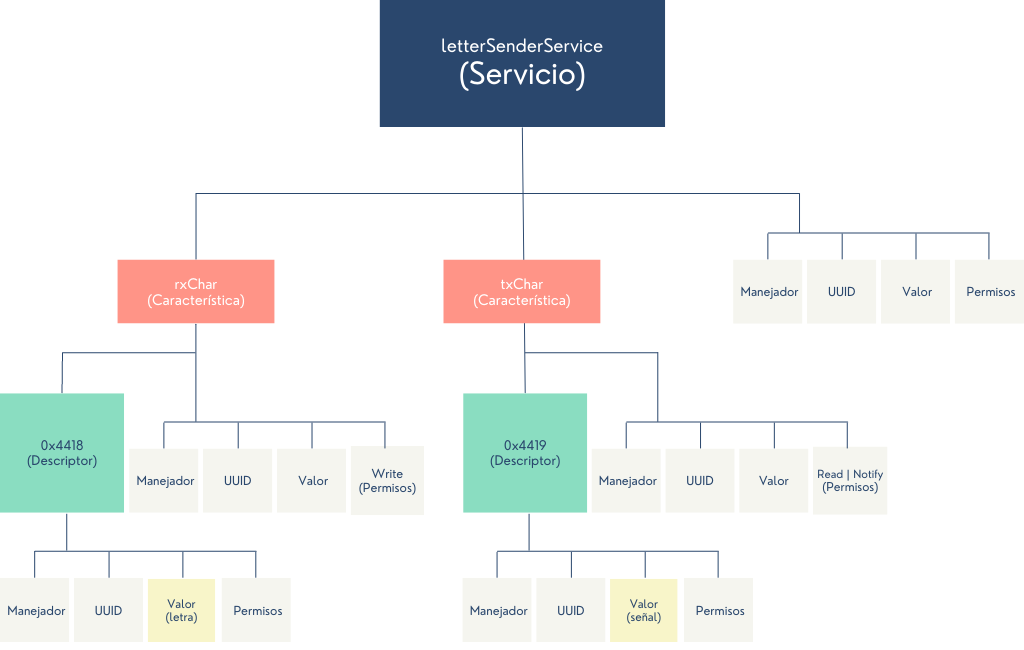
\includegraphics[width=1\textwidth]{capturas/BleLetterSenderService.png}\\[-0,40cm]
    \caption{Esquema de la estructura planteada para el servicio \textit{BLE}}
\end{figure}

\section{Implementación}
Previo a la implementación del código, se deben instalar ciertas librerías
(proceso sencillo gracias a la decisión de utilizar el \textit{Arduino IDE}
pero que puede consultarse en el apéndice \ref{libArduino})
para el trabajo con algunas características de la \textit{Arduino Nano Sense 33 BLE}
como lo son la librería \textit{Arduino\_LSM9DS1}, para el uso de la IMU y su
acelerómetro, magnetómetro y giroscopio; y la librería \textit{ArduinoBLE},
para el uso del \textit{Bluetooth} de bajo consumo. Por otro lado, también
es necesario instalar la librería \textit{Arduino\_TensorFlowLite}, para
trabajar con el modelo de la red neuronal en el firmware del microcontrolador.

Además, en ocasiones, es necesario dar permisos al puerto del microcontrolador
como reza el \textit{apéndice \ref{pserie}}
\subsection{Definición de parámetros de \textit{Bluetooth}}
En el primer bloque del firmware, encontramos definición de los parametros
que más tarde se utilizarán para configurar el \textit{BLE}
(Bluetooth Low Energy)\textsuperscript{\cite{ladvien}}\label{paramBT}.

La configuración de permisos de las características son consecuentes con
su cometido. La característica de lectura, tendrá permisos de escritura
para que la \textit{central} pueda escribir los valores que la placa leerá.
Análogamente la característica de escritura tendrá permisos de lectura y
notificación.

\begin{teoria}{Roles de las partes en conexiones \textit{bluetooth}\textsuperscript{\cite{BLEOreilly}}}
    \color{mitexto}
    Al darse una conexión bluetooth, existen ciertas implicaciones inherentes
    a la propia conexión. Y es que siempre habrá una de las partes que
    se lucra de los servicios de la(s) otra(s).\\
    Pues bien, los dispositivos que se gestionan o se benefician de los
    servicios de otros, se conocen como \textit{central} y los que proveen,
    son los \textit{periféricos}.
\end{teoria}
El resultado de la configuración del servicio \textit{BLE} obedece completamente
al diseño planteado.

Finalmente se deben definir una serie de manejadores para gestionar los
distintos eventos relacionados con el servicio \textit{BLE}. Estos manejadores
se activarán como consecuencia de suceso y se encargarán de gestionar
la respuesta a dicho suceso; concretamente respuestas a conexiones,
desconexiones o recibo de señales por el canal de lectura \textit{rx}.


\subsection{Función de configuración del firmware}
En esta sección (denominada función '\textit{setup()}' en el diseño de \textit{Arduino}),
como de constumbre, se deberá llevar a cabo el ajuste propio para la ejecución
de nuestro código\textsuperscript{\cite{andriyadimw}\cite{petewardenmw}}.

Es reseñable mencionar que el microcontrolador con el que estamos trabajando solo
posee la \textit{memoria flash} y \textit{SRAM} características de
los dispositivos de estas prestaciones. Sin embargo tenemos que almacenar
alguna información imprescindible como la red neuronal o la reserva de algunas
secciones de memoria. Para ver la solución implementada con un mayor detalle técnico,
consultar el apéndice \ref{memFlash}.
Más adelante se hará uso de la misma técnica para resolver el problema
de la integración de la red neuronal en el microcontrolador, entre otros.

\subsubsection{Configuración \textit{Bluetooth} y de sensores}
En esta primera etapa de configuración, se definirá el comportamiento de algunas
características de la placa; en primer lugar, el de la  \textit{IMU}
(\textit{Inertial Measurement Unit}), la unidad con la que trabajamos para
obtener los datos del movimiento sirviéndose de un \textit{giroscopio} y un
\textit{acelerómetro}, y por otro lado, la configuración del ya descrito,
definido y diseñado \textit{BLE} (\textit{Bluetooth Low Energy}) con
los parámetros que se definieron en la sección \ref{paramBT}.
\begin{teoria}{Por qué es necesario configurar la \textit{IMU}\textsuperscript{\cite{imuteoria}}}
    La \textit{IMU} es una parte fundamental de este proyecto, ya que es
    el dispositivo contenido en la placa que gestiona las mediciones de
    aceleración y velocidad del movimiento y que consta para ello de
    acelerómetro y giroscopio. Con la captura de estos datos, podrá rasterizarse
    una imagen que contenga el trazo descrito y con la que podremos alimentar
    la red neuronal.
\end{teoria}

\begin{problemas}{Librería Arduino\_LSM9DS1}
    \color{mitexto}
    Uno de los problemas con esta parte del código, fue que
    la librería \textit{Arduino\_LSM9DS1} necesaria para poder trabajar con
    la \textit{IMU}, tiene varias versiones.
    Al haber leído para algunos de los proyectos TFLite de
    arduino, que era recomendable utilizar su primera versión, fue la elegida.
    Sin embargo esta primera versión, no posee una de las funciones
    necesarias para trabajar con la \textit{IMU} en nuestro caso,
    que es el llenado
    contínuo de la FIFO de lectura de medidas recogidas, que por defecto
    funciona en \textit{oneShotMode}, es decir, llenado a ráfagas.
    Es necesario poder disponer de la función para trabajar en tiempo
    real con la predicción de letras y también es imprescindible para la
    recolección de muestras, como se verá más adelante.
    
    Por lo que la solución es o bien añadir manualmente la función en la
    librería, o bien actualizarla a la versión \textit{1.1.0}. Yo me he
    decantado por actualizar la librería, ya que es algo más limpio que
    editar una librería que no has programado tú mismo.
\end{problemas}

Por lo que solo resta fijar los parámetros creados para \textit{BLE},
vincular sus señales con manejadores de los eventos y hacer lo propio
con la \textit{IMU}.

Cabe destacar que adicional a la configuración \textit{BLE} descrita, también
se incorpora otro servicio con la característica \textit{strokeCharacteristic},
menos interesante de explicar, ya que utilizaré el método de recolección de
muestras de \textit{Pete Warden} para uno de los ejemplos
\textit{TFLite de Arduino}: \textit{magic\_wand}\textsuperscript{\cite{petewardenmw}}.

\subsubsection{Configuración para la red neuronal}
Parte de máxima trascendencia, ya que, es imprescindible configurar de
manera adecuada los parámetros del modelo para que el reconocimiento
se de manera óptima.\\
Una vez obtenemos el modelo definido en \textit{deep\_pen\_model\_data.cpp},
proceso que se explicará en la sección \ref{RNenμC}.

Se deben establecer las micro-operaciones que se darán en el modelo
para tener definido el repertorio en tiempo de ejecución que utilizará
nuestro interprete\textsuperscript{\cite{intro-tensor-micro}}.
Existe una alternativa que añade todas las micro-operaciones de forma genérica,
a costa de un mayor uso de memoria. Para mayor profundización en la
implementación, consultar el apéndice \ref{firmwMO}.

\begin{problemas}{Al cargar el firmware\, la placa deja de ser detectada}
    En las primeras cargas del firmware experimentando con el modelo, la placa
    dejaba de ser detectada. Lo primero que pensé es que el bootloader se había
    bloqueado. Sin embargo al restaurar la placa manualmente ({\small Pulsación
    del botón reset justo al conectar la placa}), el 'L' led de la placa,
    comenzó a parpadear; indicativo de que la placa se había restaurado.
    Por tanto solo cabía que el programa cargado era erróneo.
    Dado que tanto la compilación como la ejecución no informaban de errores,
    fue complicado dar con que este error se debía a una mala configuración
    de las microoperaciones definidas.\\Ya que al hacer cambios en el diseño
    del modelo, es imperativo añadir las microoperaciones ampliadas.
    Un error de principiante que llevó mucho tiempo arreglar.
\end{problemas}

Para finalizar la configuración de \textit{TensorFlow Lite} definimos el interprete del modelo, que hará
uso del repertorio de micro-operaciones especificadas.\newline
Y por último, inicializamos los led pins como salida, para poder hacer uso
del led como indicativo de estado.

\subsection{Función cíclica del firmware}
En esta función (denominada 'loop()' en el diseño \textit{Arduino}),
será donde se establezca el código que se ejecutará persistentemente
mientras la placa esté alimentada\textsuperscript{\cite{andriyadimw}\cite{petewardenmw}}.

En primer lugar, se tratará la lógica para los leds es simple:
\begin{figure}[h]
    \centering
    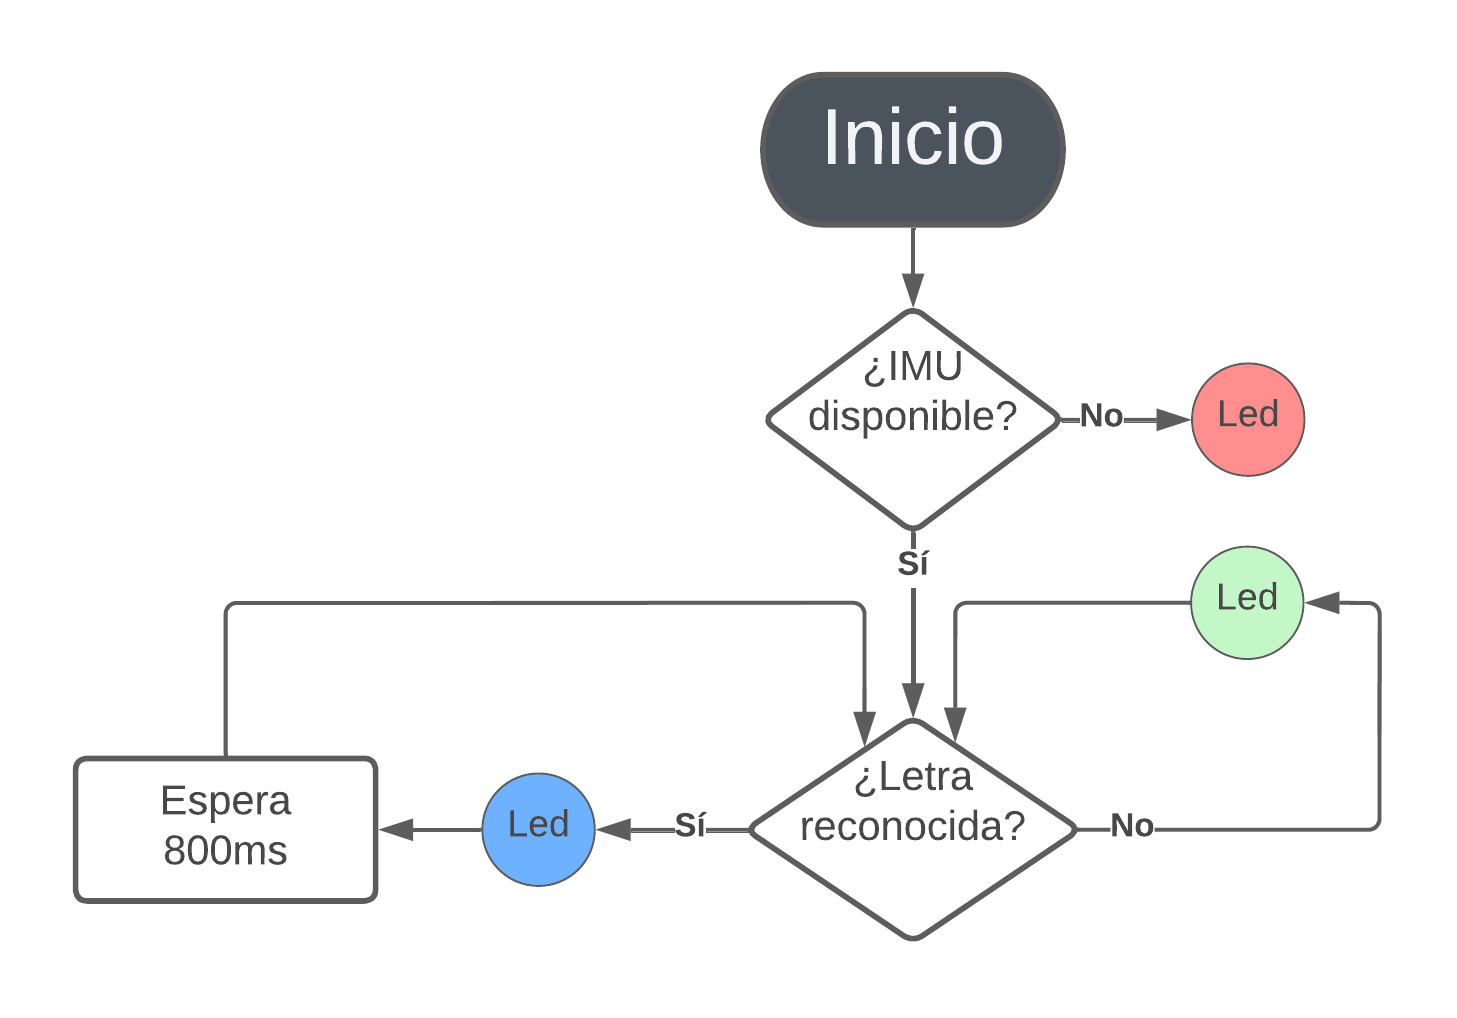
\includegraphics[width=0.82\textwidth]{capturas/DiagramaFlujoLeds.png}\\[-0,20cm]
    \caption{Diagrama de flujo de leds}
\end{figure}\\
En estado idle el led
encendido será el verde y en estado de detección de letra, será azul (quedará en este estado
durante 800ms, tiempo durante el que no se detectará nada, para que el usuario pueda
reposicionar su postura para volver a escribir otra letra); en caso de que la \textit{IMU}
no esté disponible, se encenderá el led rojo.

Para notificar una vez la conexión a un dispositivo, pese a que
la ejecución es cíclica, se implementa una sencilla solución descrita en el
apéndice \ref{BTcon}.

En cuanto al registro de movimiento, se han utilizado algunas de las funciones
del trabajo de \textit{Pete Warden} y su \textit{magic\_wand}\textsuperscript{\cite{petewardenmw}}
a modo de librería para mi propio proyecto y así aligerar el desarrollo de
la recolección de trazos y su rasterización.

Durante este proceso, se hará uso del giroscopio para determinar los cambios del trazo y el acelerometro
para pequeños ajustes sobre los resultados obtenidos con el giroscopio, por ejemplo
cálculos de gravedad y parámetros de velocidad del cambio de trayectoria del trazo.
Gracias a contar con las funciones antes citadas, tomar los valores de los sensores
es tan fácil como llamar a la función \textit{ReadAccelerometerAndGyroscope}.
Con los valores leídos, se hace un pequeño arreglo de estimación de desvío del giroscopio
y se envían los valores leídos como característica del servicio para \textit{Data Collector},
donde se recogeran las muestras para entrenar la red neuronal.
Y con el trazo completamente construido y corregido, se rasteriza el movimiento para
obtener la imagen que pasará por el modelo.

Con todo lo anterior definido, todo está listo para dar comienzo con el procesamiento
en la red neuronal. Para llamar a su ejecución,
se invoca el interprete, que arrojará los resultados en un puntero anteriormente definido.
Este puntero de salida, contiene los datos asociados al tensor, es decir, el producto
de que el trazo rasterizado haya pasado por la red neuronal. En nuestro caso, lo que
se obtiene de la red neuronal, es una valoración de ajuste de afinidad del trazo rasterizado
a lo que el modelo ha sido entrenado para reconocer como letras (nuestros \textit{labels}).\
Sintetizando, lo que se obtiene como salida de la red neuronal, es una valoración
de semejanza a cada letra, codificada como un índice.

Por tanto, lo que resta es trivial, solo tenemos que obtener el \textit{label} con mayor valoración.
Y como consecuencia, la letra que el modelo ha estimado más posible respecto a su entrenamiento.

Obtenida la letra, es enviada al puerto serie, para cuando se trabaje con conexión física;
y se introduce en la característica de transferencia(\textit{tx}) para cuando se trabaje
con el servicio \textit{Bluetooth} (\textit{BLE}).

Como comprobación concluyente, se verifica si la característica de lectura (\textit{rx}) ha sido
escrita por el programa de usuario, suponiendo esto una señal de que ya ha sido leída la letra
actual en \textit{tx} y como consecuencia, haciendo que se restaure su valor a uno por defecto;
ya que de no hacerlo, la letra permanecería inmutable en la característica y el programa
de usuario leería las mismas letras reiteradamente hasta escribir otras.
Esto se debe a que el las \textit{características} en \textit{BLE} funcionan con valores
constantes hasta que se modifique el estado actual.

\begin{figure}[h]
    \centering
    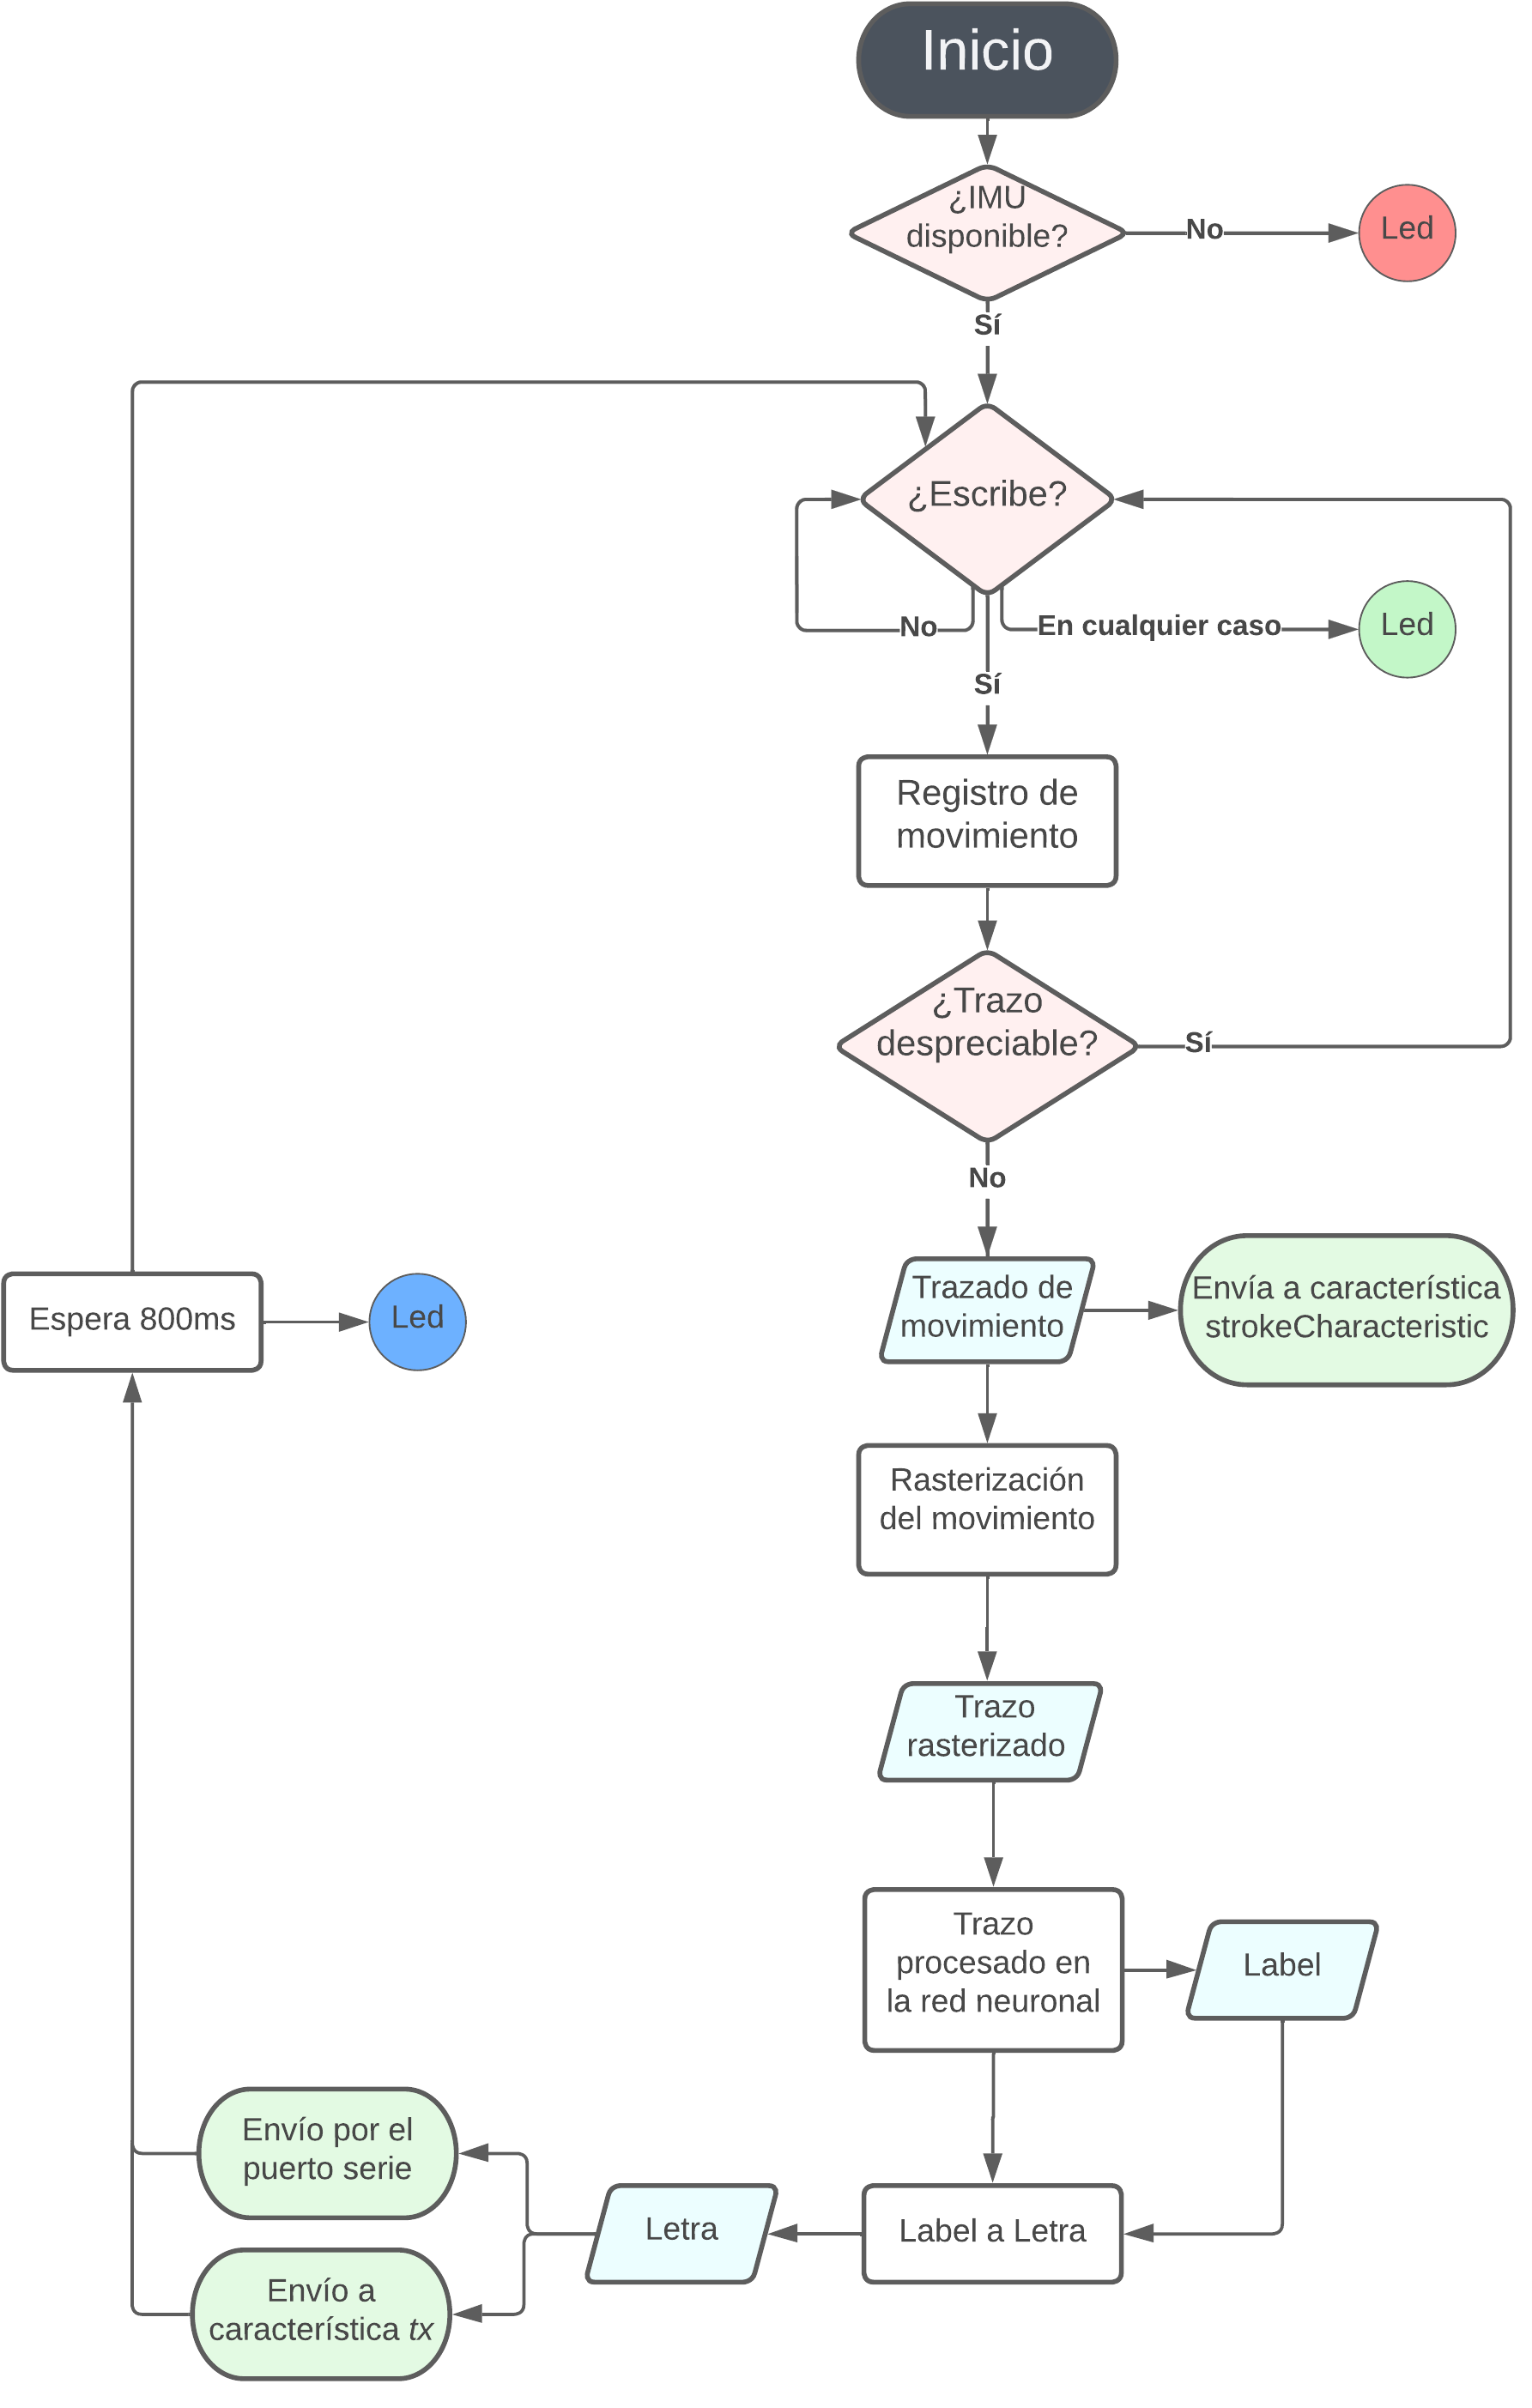
\includegraphics[width=0.8\textwidth]{capturas/DiagramaFlujoFirmware.png}\\[-0,48cm]
    \caption{Diagrama de flujo simplificado del firmware del microcontrolador}
\end{figure}